 \documentclass[book.tex]{subfiles}
\begin{document}

\section{Action Phase: Adaptive Tile Refreshment}
\label{section:adaptive_tile_refresh}
After the player is done setting up the game, it is time for the scrolling engine to shine. On bitmapped displays without hardware scrolling like the EGA card, the entire screen have to be erased and redrawn in the slightly shifted position whenever the player moved in any direction. This would kill the CPU as you need to update all pixels of all four planes on the EGA card (remember the planar mapping of section \ref{section:EGA_Planar_Madness}?).\\ 

So here John Carmack came with a smart solution. The scrolling engine is based on a simple yet powerful technology called Adaptive Tile Refreshment. The core idea is to  refresh only those areas on the screen that needed to change.\\

The visible screen is divided into tiles of 16x16 pixels. On a screen with 320x200 pixels, it means a grid of 20x13 tiles (actually it is 12.5 tiles high, but we need to round to integer). Let's look at \textit{Commander Keen 1: Marooned on Mars} in Figure \ref{fig:keen_difference}. This is the first level of Marooned, immediately to the right of the crashed Bean-with-Bacon Megarocket. The first figure is the start of the level, the second figure is after Keen has moved one tile (16 pixels) to the right through the world. They look almost identical to the naked eye, don't they? \\

Now, if we perform a difference on both images you see which tiles needs to be changed upon screen refresh. The trick behind the scrolling in the first Commander Keen games was to only redraw tiles that actually changed after panning 16 pixels (one tile), since most maps had large swathes of constant background. In case of Figure \ref{fig:keen_difference} only 69 tiles of the total 260 tiles need to be refreshed, which is 27\% of the screen! 



\pagebreak
\begin{figure}[H] 
  \centering 
  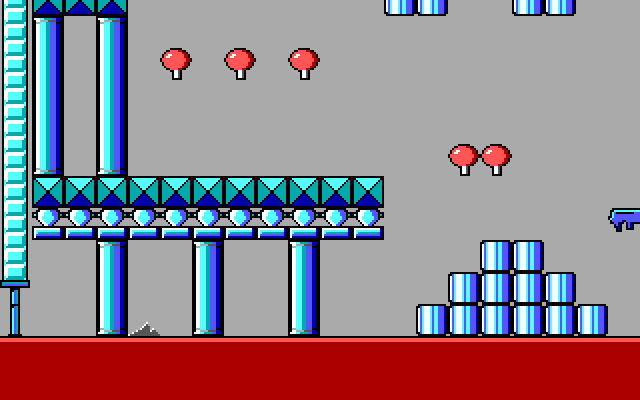
\includegraphics[width=.6\textwidth, frame]{screenshots_300dpi/game/keen-screen1.png}
\end{figure}
\begin{figure}[H] 
  \centering 
  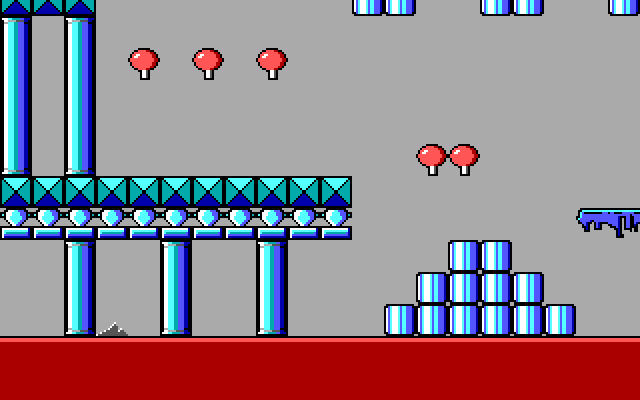
\includegraphics[width=.6\textwidth, frame]{screenshots_300dpi/game/keen-screen2.png}
\end{figure}
\begin{figure}[H] 
  \centering 
  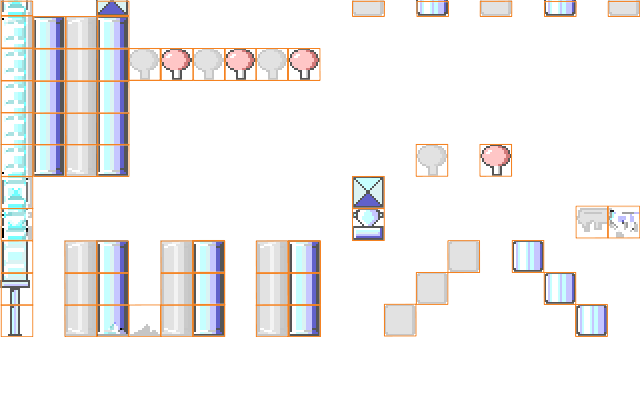
\includegraphics[width=.6\textwidth, frame]{screenshots_300dpi/game/keen-difference.png}
  \caption{Start of the world, moved one tile to the right and difference.}
  \label{fig:keen_difference}
\end{figure}
\pagebreak

So now we know how to scroll the screen in steps of 16 pixels, which is still pretty 'choppy'. For smooth scrolling we need to dive deeper into the EGA card, which is explained in the next section.\\


\subsection{EGA Virtual Screen}
\label{section:EGA_virtual_screen}

The EGA adds a powerful twist to linear addressing: the logical width of the virtual screen in VRAM memory need not to be the same as the physical width of the screen display. The programmer is free to define a logical screen width of up to 4096 pixels and then use the physical screen as a window onto any part of the virtual screen. What's more, a virtual screen can have any logical height up to the capacity of the VRAM memory. The code below illustrates how to change the logical width.\\

\begin{minipage}{\textwidth}
  \lstinputlisting[language=C]{code/SCREEN_WIDTH.ASM}
  \end{minipage}
  \label{ega_pel_pan}
  \par

The area of the virtual screen displayed at any given time is selected by setting the display memory address at which to begin fetching video data. This is set by way of the CRTC Start Address register. The default address is \cw{A000:0000h}, but the offset can be changed to any other number. In EGA's planar graphics modes, the eight bits in each byte of video RAM correspond to eight consecutive pixels on-screen. Panning down a scan line requires only that the start address is increased by the logical width in bytes. Horizontal panning is possible by increasing the start address by one byte, although in this case only relative coarse of 8 pixels (1 byte)  adjustments are supported. See the code below how to set the CRTC Start Address register.

\begin{minipage}{\textwidth}
  \lstinputlisting[language=C]{code/EGA_SET_ADDRESS.ASM}
  \end{minipage}
  \label{ega_set_address}
  \par

\subsection{Horizontal Pel Panning}
Smooth pixel scrolling of the screen is provided by the Horizontal Pel Panning register in the Attribute Controller (ATC). Up to 7 pixels' worth of single pixel panning of the displayed image to the left is performed by increasing the register from 0 to 7. \\
\par

There is one annoying quirk about programming the Attribute Controller: when the ATC Index register is set, only the lower five bits (bits 0-4) are used as the internal index. The next most significant bit, bit 5, controls the source of the video data send to the monitor by the EGA card. When bit 5 is set to 1, the ouput of the palette RAM controls the displayed pixels; this is normal operation. When bit 5 is 0, video data doesn't come from the palette RAM, and the screen becomes a solid color. To ensure the ATC index register is restored to normal video, we must set bit 5 to 1 by writing \cw{20h} to the register.\\ 

\begin{minipage}{\textwidth}
  \lstinputlisting[language=C]{code/EGA_PELPAN.ASM}
  \end{minipage}
  \label{ega_pel_pan}
  \par

\subsection{Smooth scrolling: Bring it all together}
Now we know how to perform tile refresh and smooth scrolling, it is time to bring it all together. The game and all actors are defined in a global coordinate system, which is scaled to 16 times a pixel. The higher resolution enables more precision of movements and better simulation of movement acceleration. Conversion between global, pixel and tile coordinate systems can be easily performed by bit shift operations:
\begin{itemize}
\item From global to pixel is shifing 4 bits to right.
\item From pixel to tile is shifting 4 bits to right.
\item From global to tile is shifting 8 bits to right.
\end{itemize}

The idea is to first perform all actions and movements in the global coordinate system, and then translate back to pixel or tile coordinate system for video updates. \\
\begin{minipage}{\textwidth}
  \lstinputlisting[language=C]{code/EGA_REFRESH.ASM}
  \end{minipage}
  \label{ega_refresh}
  \par


So the smooth horizontal and vertical panning should be viewed as a series 16-pixel tile refreshment and fine adjustments in the 8-pixel range. The scrolling is defined by the following steps, see also Figure \ref{fig:tile_refresh}:
\begin{itemize}
  \item Calculate the panning in pixels for both x- and y-direction
  \item The y-panning is defined by adding \cw{logical width * y} to the CRTC start address
  \item In case the panning in x-direction is more than 8 pixels, increase the CRTC start address by 1 byte. This is where we need \cw{pansx}.
  \item the remaining pixels, ranging from 0-7, will be adjusted using horizontal pel panning
\end{itemize}


\begin{figure}[H]
\centering
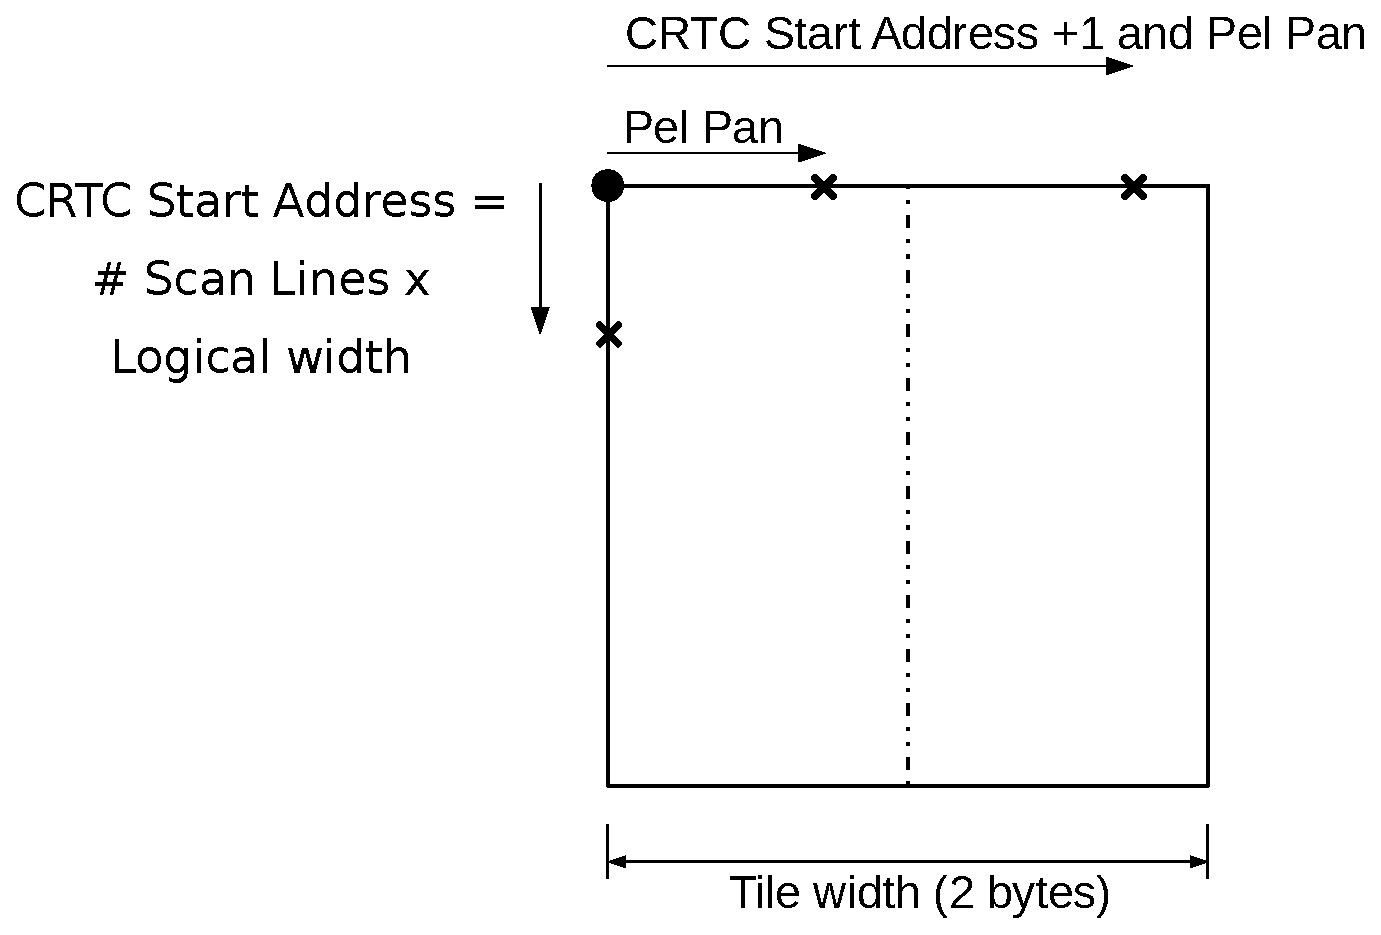
\includegraphics[width=0.6\textwidth]{imgs/drawings/Tile_Refresh.eps}
\caption{Smooth scrolling in EGA.}
\label{fig:tile_refresh}
\end{figure}





\section{View Port and Buffer setup}
Before explaining the scrolling algoritm, let's first explain how the view port and buffer layout are setup. The visible viewing screen on EGA has a resolution of 320x200 pixels. Translated in 16x16 pixel tiles, the screen view has a size of 20x13 tiles. By making the view port one tile higher and wider than the screen, the engine can scroll the screen up to 16 pixels to the right or bottom side of the screen without any tile refresh, by means of adjusting the CRTC Start Address and Pel Pan registers. Finally, the buffer must have enough space to float the view port up to two tiles in all direction. At the end of Section \ref{section:scroll_refresh_dreams} it is explained why we need a spare buffer of 2 tiles.\\

So summarized, as illustrated in Figure \ref{fig:screen_setup}, the following tile views are defined:
\begin{itemize}
\item Screen View size of 20x13 tiles and Port View size of 21x14 tiles.
\item Buffer screen size of 22x14 tiles. This is one tile wider than the Port View, where the additional tile is used to mark a '0' at the end of each tile row. 
\item Total buffer is the buffer screen plus two times a spare buffer to support floating the buffer screen two tiles in any direction.
\end{itemize}
\par
 
\begin{figure}[H]
\centering
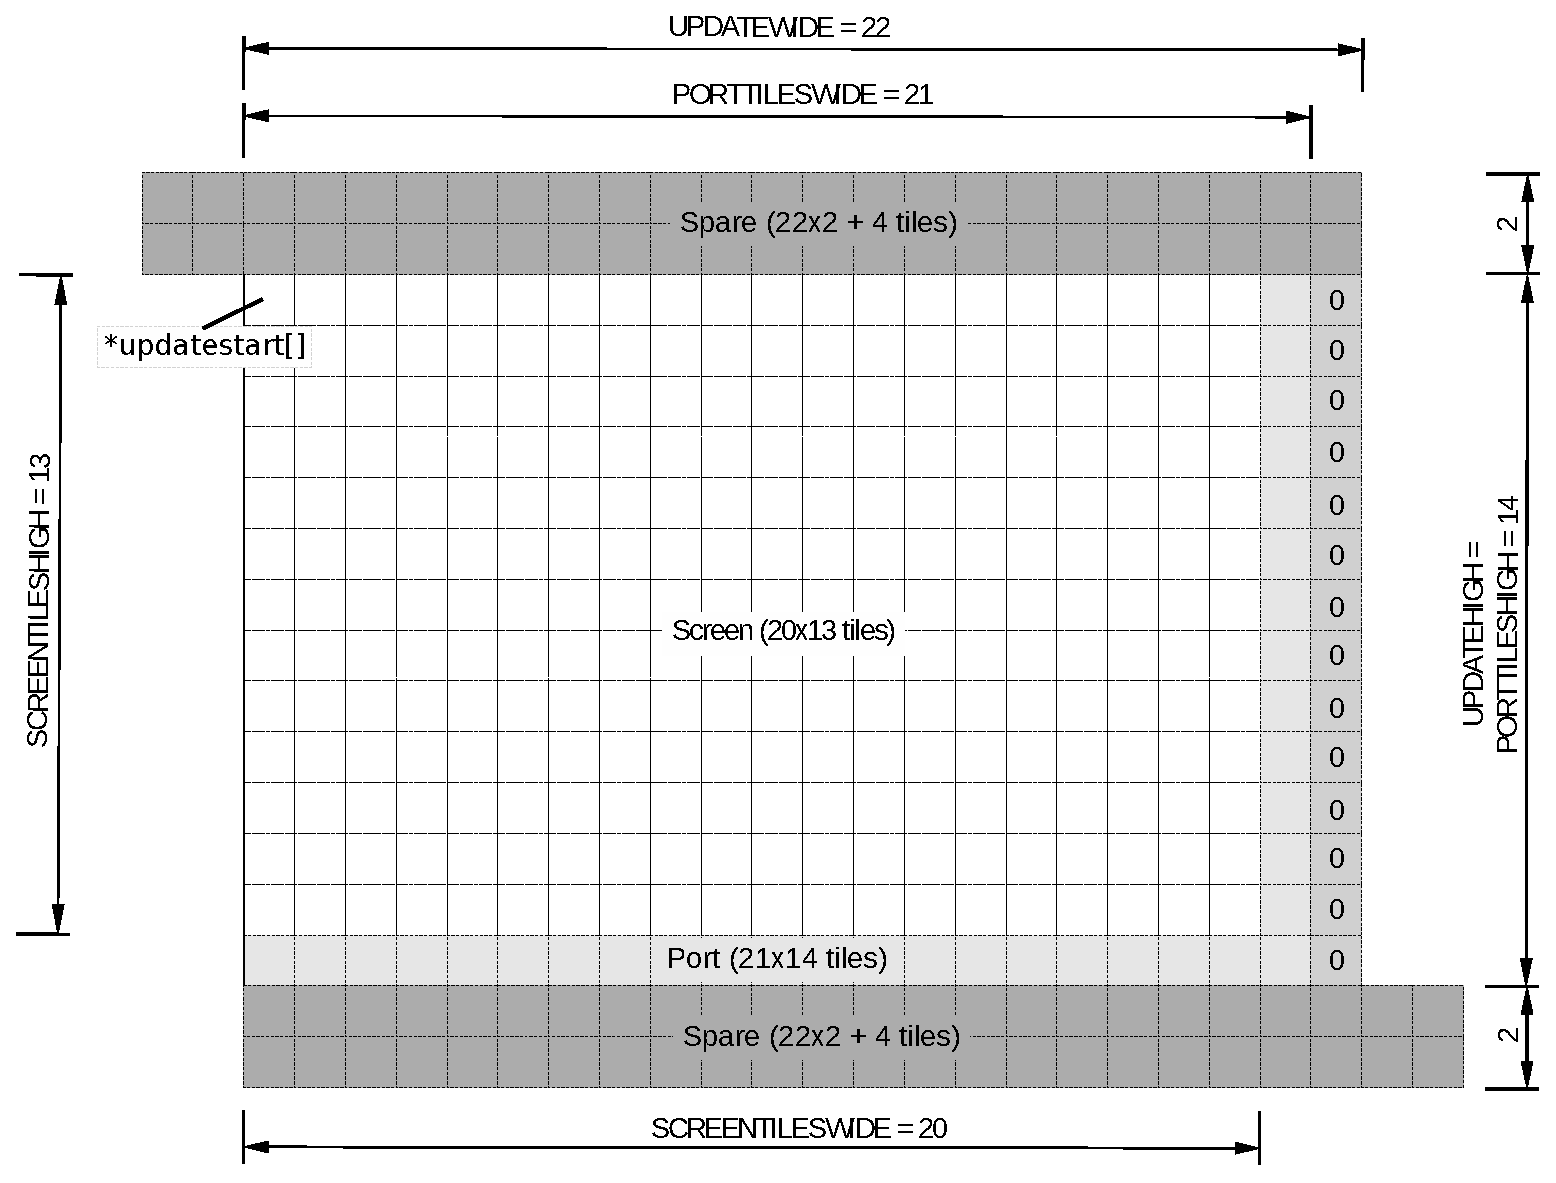
\includegraphics[width=\textwidth]{imgs/drawings/buffer_tile_layout.eps}
\caption{View and buffer tile layout.}
\label{fig:screen_setup}
\end{figure}



\section{Virtual screen buffer}
Even if the screen is not scrolling, tile refreshes are required to support sprite animations. Since moving a sprite in this way involves first erasing it and then redrawing it, the image of the erased sprite may be visible briefly, causing flicker. This is where double buffering comes in: setting up a second buffer into which the code can draw while the first buffer is being shown on screen, which is then switched out during screen refresh. This ensures that no frame is ever displayed mid-drawing, which yields smooth, flicker-free animation.\\

Now, let's have a closer look at the EGA memory setup. As explained in the previous section, the view port has a size of 21x14 tiles, which is 336x224 pixels. That means the logical width in VRAM must be at least 336 pixels (42 bytes) wide. In the file \cw{id\_vw.h} the VRAM screen buffer is defined by SCREENSPACE, which is set to 64x240 bytes, or 512x240 pixels. This is more than sufficient to update one virtual screen in VRAM.\\

Since one screen only uses 15,360 bytes of VRAM (which is 3,840 bytes per plane), there is more than enough space to store more than two full screens of video data. The video memory is organized into three virtual screens:
\begin{itemize}
\item Page 0 and 1, which are used to switch between buffer and view screen
\item A master page containing a static page, which is copied to the buffer memory when performing the screen refresh.
\end{itemize}
\par

\begin{figure}[H]
\centering
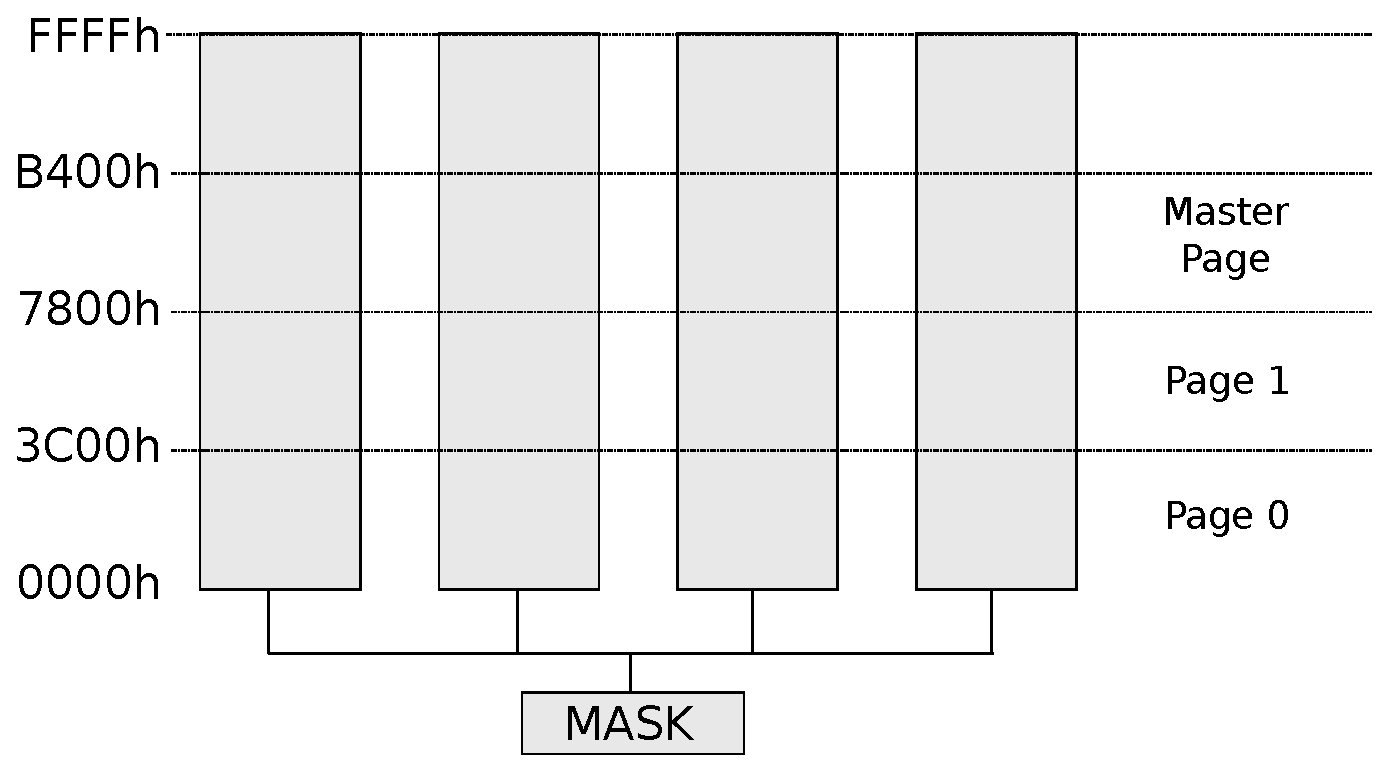
\includegraphics[width=\textwidth]{imgs/drawings/ega_ram_architecture.eps}
\caption{Virtual screen layout on EGA card.}
\label{fig:ega_ram_arch}
\end{figure}

The page that is actually displayed at any given time is selected by setting the CRTC Start Address register at which to begin fetching video data.\\




\section{Life of a 2D Frame}
The approach of refreshing the screen is different between the first Commander Keen games, Commander Keen 1-3, and the ones after. In the first games the algoritm keeps the view and buffer screen at fixed VRAM locations, where it performs a check which tiles are changed after the scroll. In the later games, it makes use of the moving the VRAM location and add a full row or column at the beginning or end of the view port. 
\\
\subsection{Adaptive tile refreshment in Commander Keen 1-3}
In the this section we explain how the first 3 versions of the game are working\footnote{We can only explain how the algoritm is working without code examples, since the only released code is Keen Dreams which is using the improved algoritm.}. Six stages are involved in drawing a 2D scene:
\begin{enumerate}
\item Check if the player has moved one tile in any direction.
\item Validate which tiles have changed (both from scrolling and animated tiles), copy these respective tiles to the Master screen and mark the tiles to be updated upon the next refresh for both pages (view and buffer screen).
\item Refresh the buffer screen by scanning all tiles. If a tile needs to be updated, copy the tile from the master screen to the buffer screen.
\item Iterate through the sprite removal list and copy corresponding image block from the master screen to buffer screen. 
\item Iterate through the sprite list and copy corresponding sprite image block from asset location in RAM to buffer screen.
\item Switch the view and buffer screen by adjusting the CRTC Start Address and Pel Panning registers.
\end{enumerate}

Before we start the explanation, let's first describe the most important variables and definitions used for the refresh process:
\begin{itemize}
  \item \cw{screenstart[]} is a pointer to the starting address (upper-left pixel) of the viewport in VRAM. As explained before we maintain three viewports in VRAM:
  \begin{itemize}
    \item screenpage, the active displayed screen on the monitor. Note that the engine never works or updates the active screen.
    \item otherpage, which is the buffer screen. This screen is updated and will be switched with the screenpage upon next refresh.
    \item masterpage, which stores a complete static background, without sprites. This page is used to update the buffer screen.
  \end{itemize}
  \item \cw{updatestart[]} is a pointer to the tile buffer array. It maintains which tiles needs to be updated upon next refresh. There are two tile buffer arrays; one for the screenpage and one for otherpage.
  \item \cw{Visible screen}, which refers to the starting position of the visible screen on the monitor. This is done by setting both the \cw{CRTR} start address and \cw{Pel Panning}. 
\end{itemize}

In the next six screenshots, we take you step-by-step through each of the stages. The player has moved and forces the screen to scroll one tile to the right. \\

\begin{figure}[H]
\centering
 \fullimage{/game/Scroll_KC1-3_1.png}
 \caption{Step 1: Scroll screen to the right}
 \label{fig:kc1_3_start}
\end{figure}

\begin{figure}[H]
\centering
 \fullimage{/game/Scroll_KC1-3_1-mem2master.png}
 \caption{Step 2: Update changed tiles in masterscreen, marked in dark grey}
 \label{fig:kc1_3_update_masterscreen}
\end{figure}

Each tile of the buffer screen is compared with the corresponsing tile on the view screen. If the tile number has changed, the tile needs to be updated by copying tile data from the asset location into the corresponding location of the masterpage.\\
\par
In parallel both the tile buffer and tile view array the changed tiles are marked with a '1', which means it needs to be updated upon next refresh.

\begin{figure}[H]
\centering
 \fullimage{/game/Scroll_KC1-3_1-tile_mem2master.png}
 \caption{Mark all changed tiles with '1' in both tile buffer and tile view array.}
 \label{fig:kc1_3_update_refresh_img_1}
\end{figure}


\pagebreak

\begin{figure}[H]
\centering
 \fullimage{/game/Scroll_KC1-3_1-master2buffer.png}
 \caption{Step 3 and 4: Copy tiles from master to buffer screen and remove sprites}
 \label{fig:kc1_3_update_remove}
\end{figure}

The next step is to scan all tiles in the tile buffer array and for each tile marked as '1', copy the tile from master to buffer screen.\\
\par
If a sprite has moved, the previous sprite location is added to the block removal list. For each block in this removal list, erase the sprite by copying the width and height of the sprite block (marked in green in Figure \ref{fig:kc1_3_update_remove}) from the master screen to the buffer screen, and mark the corresponding tiles only in the tile buffer array with a '2'.

\begin{figure}[H]
\centering
 \fullimage{/game/Scroll_KC1-3_1-tile_master2buffer.png}
 \caption{Mark removed sprites with '2' in tile buffer array only.}
 \label{fig:kc1_3_tile_update_remove}
\end{figure}


\pagebreak

\begin{figure}[H]
\centering
 \fullimage{/game/Scroll_KC1-3_1-sprite2buffer.png}
 \caption{Step 5: Scan sprite list and copy sprite onto buffer screen}
 \label{fig:kc1_3_update_sprite}
\end{figure}

Next, the engine scans the sprite list. Validate if the sprite is in the visible part of the view port and copy the sprite image to the buffer screen. Mark the corresponding tiles in the tile buffer array with a '3'.

\begin{figure}[H]
\centering
 \fullimage{/game/Scroll_KC1-3_1-tile_sprite2buffer.png}
 \caption{Mark new sprites locations with '3' in tile buffer array only.}
 \label{fig:kc1_3_tile_update_sprite}
\end{figure}


\pagebreak


\begin{figure}[H]
\centering
 \fullimage{/game/Scroll_KC1-3_1-final.png}
 \caption{Step 6: Swap buffer and screen page}
 \label{fig:kc1_3_update_final}
\end{figure}


As the final step, point the visible screen to the buffer screen by updating the CRTR start address and horizontal Pel Panning register. The entire tile buffer array is then cleared to '0'. Finally the otherpage and screenpage of both the \cw{screenstart[]} and \cw{update[]} are swapped. Then step 1 is repeated. \\
\par
Note that after swapping, the tile buffer array still has marked all tiles that have changed from scrolling the screen. This makes sense as the current buffer screen is not yet updated (it was displayed in the previous cycle, and we never update the view screen). 

\begin{figure}[H]
\centering
 \fullimage{/game/Scroll_KC1-3_1-tile_final.png}
 \caption{Clear tile update array and swap arrays.}
 \label{fig:kc1_3_tile_final}
\end{figure}


\pagebreak

\begin{figure}[H]
\centering
 \fullimage{/game/Scroll_KC1-3_1_final.png}
 \caption{Step 6: Swap buffer and screen page}
 \label{fig:kc1_3_update_final}
\end{figure}

Step 2 and 3 (except for the animated tiles) only needs to happen if Commander Keen is moving more than 16 pixels, where step 4 and 5 normally needs to happen for each refresh.
So the number of drawing operations required during each refresh is controllable by the level designer. If they choose to place large regions of identical tiles (the large swathes of constant background), less redrawing (meaning: less redrawing in step 2 and 3) is required.

\pagebreak

\subsection{Optimize tile updates}
\label{section:optimize_tile}
The hardware chapter described Mode \cw{0Dh}, which despite being unfit for games, still has an interesting characteristic. As explained in Section \ref{section:ega_memmap} each pixel is encoded by four bits, which are spread across the four EGA banks. Since all write operations are one byte wide, it is not hard to imagine the difficulty in plotting a single pixel without changing the others stored in the same byte. One would have to do four read, four xor, and four writes.\\
\par
 Since the designers of the EGA were not complete sadists, they added some circuitry to simplify this operation. For each bank, they created a latch placed in front of a configurable ALU.\\
\par
 \begin{figure}[H]
\centering
 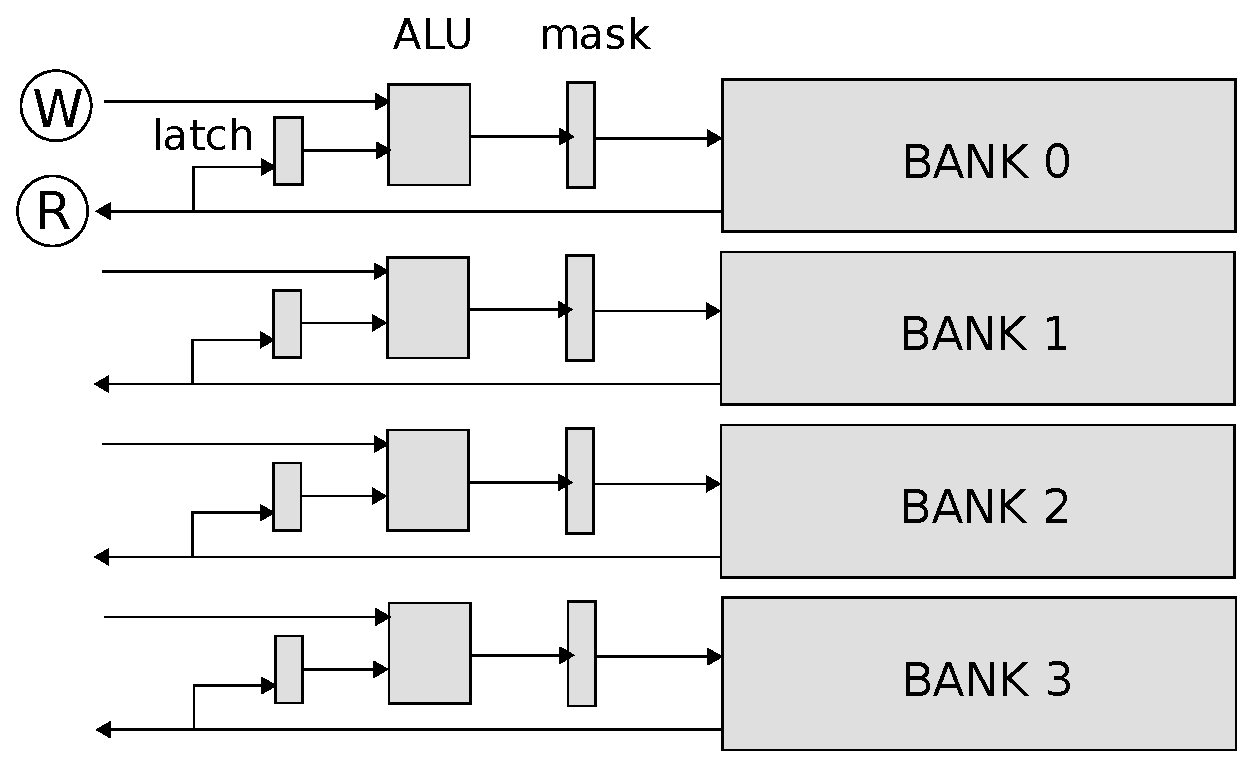
\includegraphics[width=\textwidth]{imgs/drawings/latches.eps}
 \caption{Latches memorize read operations from each bank. The memorized value can be used for later writes.}
 \end{figure}
With this architecture, each time the VRAM is read \circled{R}, the latch from the corresponding bank is loaded with the read value. Each time a value is written to the VRAM \circled{W}, it can be composited by the ALU using the latched value and the written value. This design allowed mode \cw{0Dh} programmers to plot a pixel easily with one read, one ALU setup, and one write instead of four reads, 4 xors, and 4 writes.\\
\par
By getting a little creative, the circuitry can be re-purposed. The ALU in front of each bank can be setup to use only the latch for writing. With such a setup, upon doing one read, four latches are populated at once and four bytes in the bank are written with only one write to the RAM. This system allows transfer from VRAM to VRAM 4 bytes at a time.\\
\par
\begin{minipage}{\textwidth}
  \lstinputlisting[language=C]{code/EGA_LATCH_COPY.ASM}
  \end{minipage}
  \label{ega_latch_copy}
  \par

To take full advantage of this optimization, the refresh algoritm maintains a list of tiles that are already copied on the masterpage via \cw{tilecache} variable. If a tile is already on the master screen the algoritm copies the tile from that location to its destination instead of the RAM location in memory, saving the four separated writes to each memory plane.


\subsection{Wrap around the EGA Memory}
In the later versions of Commander Keen, John Carmack explored what would happen if you push the virtual screen over de 64kB, or \cw{0xFFFF}, border in video memory. It turned out that the EGA continues the virtual screen at \cw{0x0000}. This means you could wrap the virtual screen around  the EGA memory and only need to add a stroke of tiles on one of the edges when Commander Keen moves more than 16 pixels.\\
\par
\begin{figure}[H]
  \centering
  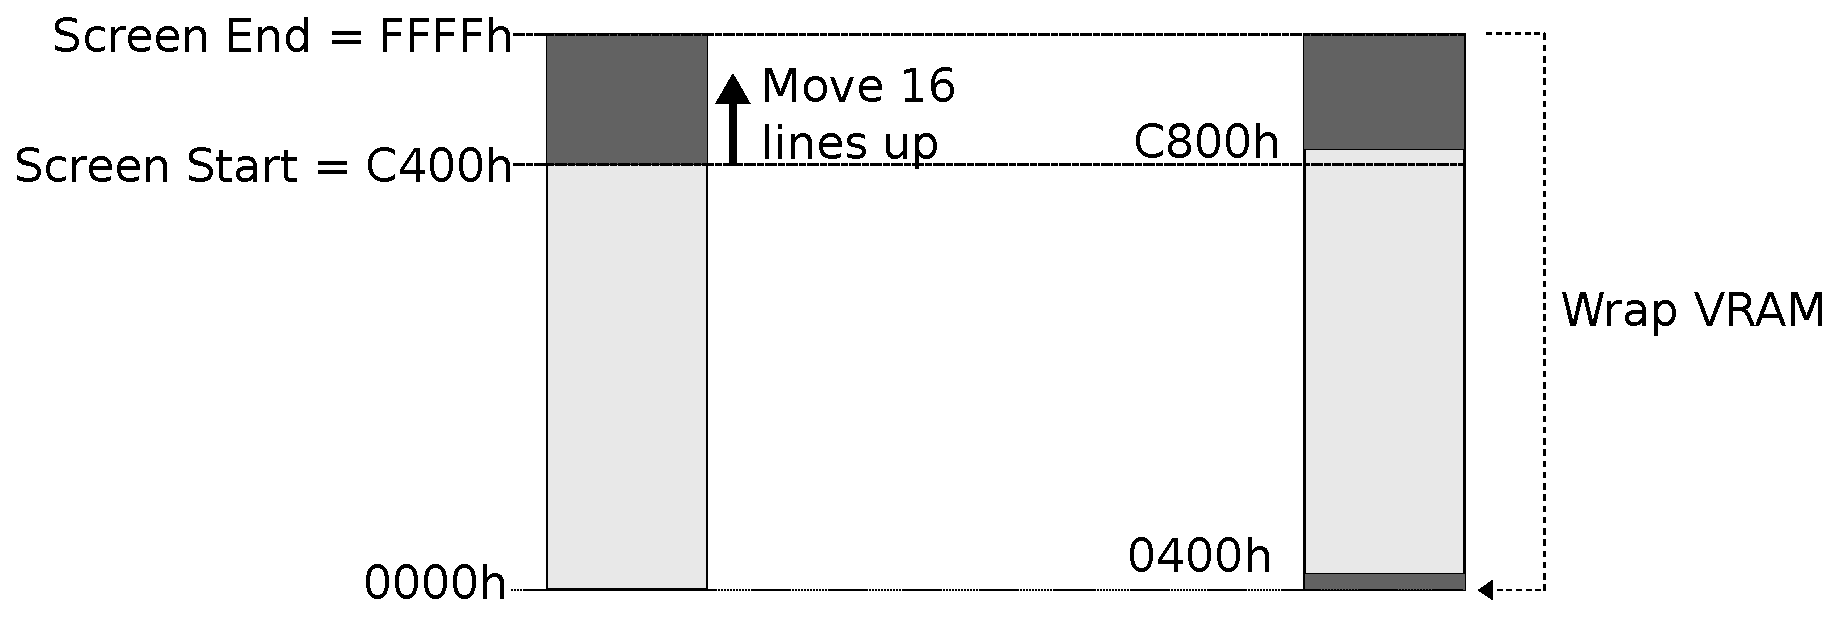
\includegraphics[width=\textwidth]{imgs/drawings/ega_wrapping.eps}
  \label{fig:ega_wrapping}
  \caption{Wrap virtual screen around the EGA memory}
\end{figure}
\par
There was however an issue with the introduction of Super VGA cards, which had typically more than 256kB RAM\footnote{In 1989 the VESA consortium standardized an API to use Super VGA modes in a generic way. One of the first modes was 640x480 at 256 colors requiring at least 256kB RAM, which from a hardware constraint resulted in 512kB.}. This resulted in crippled backwards compatibility and the wrapping around \cw{0xFFFF} did not work anymore on these cards. \\
\par
Luckily there was a way to resolve this issue. As you can see in Figure \ref{fig:ega_ram_arch} on page \pageref{fig:ega_ram_arch}, the space between \cw{0xB400} and \cw{0xFFFF} is not used and contains enough space for another virtual screen. Each screen buffer has a size of \cw{0x3C00} in each memory bank. In case the start address is between \cw{0xC400} and \cw{0xFFFF} the corresponsing screen is copied to the opposite end of the buffer, as illustrated in Figure \ref{fig:page_wrapping}.\\
\par
\begin{figure}[H]
\centering
\begin{subfigure}{.5\textwidth}
  \centering
  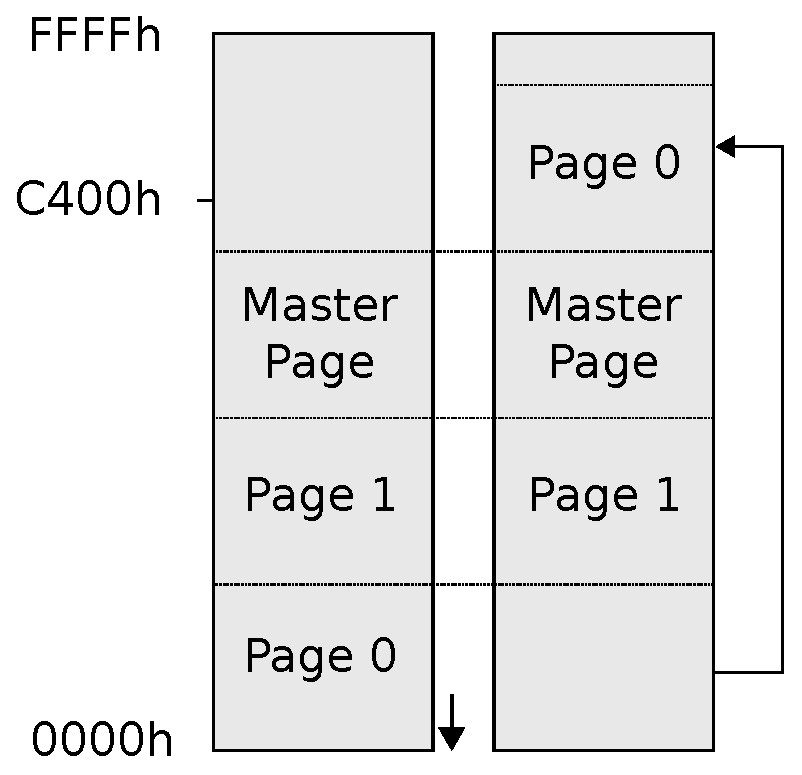
\includegraphics[width=.9\textwidth]{imgs/drawings/Page_down_switch.eps}
  \caption{Virtual pages moved down}
  \label{fig:page0_down}
\end{subfigure}%
\begin{subfigure}{.5\textwidth}
  \centering
  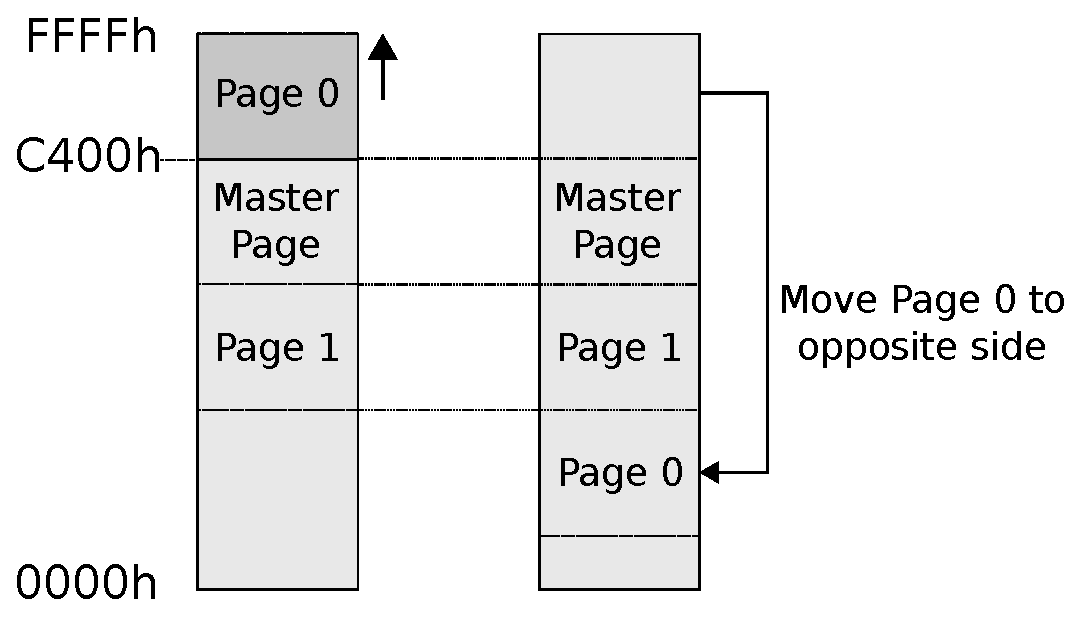
\includegraphics[width=.9\textwidth]{imgs/drawings/Page_up_switch.eps}
    \caption{Virtual pages moved up}
  \label{fig:page0_up}
\end{subfigure}
\caption{Move screen to opposite end of VRAM buffer}
\label{fig:page_wrapping}
\end{figure}
\par
The screen copy comes at the cost of some performance, but is not noticed during game play, also due to the fact that we can make use of copying 4 bytes in one cycle using the latches as explain in section \ref{section:optimize_tile}.\\
\par
\begin{minipage}{\textwidth}
  \lstinputlisting[language=C]{code/wrap_page_buffer.c}
  \end{minipage}
  \label{ega_refresh}
  \par

Flipping between the pages is as simple as setting the CRTC start address registers to page 0 or page 1 starting point, as explained in Section \ref{section:EGA_virtual_screen}. 
However, there is one issue to solve. If you were to run it, every once in a while the expected screen shown below...

 \begin{figure}[H]
\centering
 \scaledimage{0.95}{/game/full_screen.png}
 \end{figure}
...would instead appear distorted:\\
\par
 \begin{figure}[H]
\centering
 \scaledimage{0.95}{/game/crtc_scanstart_problem.png}
 \end{figure}
\par
This glitch shows both misalignment and parts of two pages. This problem has to do with the timing between updating the CRTC starting address and screen refresh. The start address is latched by the EGA's internal circuitry exactly once per frame, typically at the start of the vertical retracement. The CRTC starting address is a 16-bit value but the \cw{out} instruction can only write 8 bits at a time. \\
\par

Now we have the following situation, where the current CRTC start address is pointing to 0x0000. We moved one tile to the left and now Page 0 is pointing at 0xFFFE in VRAM and Page 1 is at 0x3BFE. Page 1 is the updated buffer and will be displayed upon next refresh cycle. Poor timing of the vertical retracement and start address update results in the CRTC picking up a value of 0x3B00 instead of 0x3BFE:\\

\par
\begin{minipage}{\textwidth}
\lstinputlisting[language={[x86masm]Assembler}]{code/pageflip_error.c}
\end{minipage}
\par

The most obvious option is to update the start address when we pick up the vertical retracement signal via the Input Status 1 Register (bit 3 of \cw{0x3DA}). Unfortunately, by the time the vertical retrace status is observed by a program, the start address for the next frame has already been latched, having happened the instant the vertical retrace pulse began.\\

\par
The trick is to update the start address sufficient far away from when the vertical retracement starts. So we're looking for a signal that tells us it just finished a horizontal or vertical retrace and started a scan line, far enough away from vertical retrace so we can be sure the new start address will get used at the next vertical sync. This signal is provided by the Display Enable status via the Input Status 1 Register, where a value of 1 indicates the display is in a horizontal or vertical retracement\footnote{Documentation is a bit unclear here. The IBM technical documentation for VGA explains retrace takes place when bit 0 of the Input Status Register 1 is set to high ('1'). The IBM technical EGA documentation explains the opposite, saying when bit 0 is set low ('0') a retrace is taking place. For now, we assume source code and VGA documentation is correct, retrace takes place on a '1'.}.
\\

\begin{figure}[H]
  \centering
  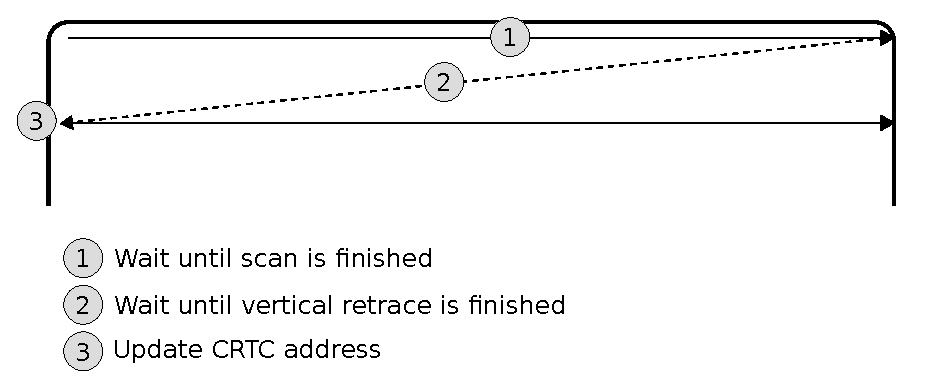
\includegraphics[width=\textwidth]{imgs/drawings/update_start_address.eps}
  \label{fig:update_start_address}
  \caption{Update CRTC start address at beginning of new scan line.}
\end{figure}
\par

Once the Display Enable status is observed, the program sets the new start address, waits for vertical retrace to happen, sets the new pel panning state, and then continues drawing.\\
\par
\begin{minipage}{\textwidth}
\lstinputlisting[language={[x86masm]Assembler}]{code/screen_refresh.c}
\end{minipage}
\par

\subsection{Scroll and screen refresh in Keen Dreams} \label{section:scroll_refresh_dreams}

The EGA memory wrapping results in the following improved algoritm to scroll and refresh the screen for Keen Dreams:
\begin{enumerate}
\item Check if the player has moved one tile in any direction.
\item In case the player moved one tile, move the \cw{screenstart[]} pointers accordingly. 
\item Copy the new introduced column or row of tiles to the Master screen and flag this new column/row of tiles to be updated in the next refresh for both pages. 
\item Refresh the buffer screen by scanning all tiles in the tile buffer array. If a tile is flagged for update, copy the tile from the master screen to the buffer screen.
\item Iterate through the sprite removal list and copy corresponding image block from master screen to buffer screen. 
\item Iterate through the sprite list and copy corresponding sprite image block from asset location in RAM to buffer screen.
\item Switch the view screen and buffer screen by adjusting the CRTC Start Address and Pel Panning register.
\end{enumerate}

As you can see, step 2 to 4 are different from Commander Keen 1-3, the rest of the steps are the same. In the example below the screen is forced to scroll to the left.
\\

\begin{figure}[H]
\centering
 \fullimage{/game/Scroll_KC4_6_1.png}
 \caption{Step 1: Scroll screen to the left}
 \label{fig:kc4_6_start}
\end{figure}

\begin{figure}[H]
\centering
 \fullimage{/game/Scroll_KC4-6_1-mem2master.png}
 \caption{Step 2 and 3: Shift screen pointer and add column to VRAM}
 \label{fig:kc4_6_add_column}
\end{figure}


First decrease the \cw{screenstart[]} of all three screen locations 2 bytes (1 tile). Then copy a left-column of tiles from the asset or cache location into the corresponding location of the masterscreen.\\
\par
In parallel decrease both the tile buffer and tile display array pointers one byte and mark each tile on the left border in both buffer arrays with '1', so it is updated upon the next refresh.
Finally, the most right column (which is now outside the view port) is marked with a '0'.

\begin{figure}[H]
\centering
 \fullimage{/game/Scroll_KC4-6_1-tile_master2buffer.png}
 \caption{Mark new column in both tile buffer and display array.}
 \label{fig:kc4_6_tile_final}
\end{figure}


\begin{figure}[H]
\centering
 \fullimage{/game/Scroll_KC4-6_1-sprite2buffer.png}
 \caption{Step 4 and 5: Copy master to buffer screen and remove sprites}
 \label{fig:kc4_6_update_buffer}
\end{figure}



Just like before, we copy the animated tiles from asset or cache location to master screen and mark them as '1' in both tile arays. Then we scan all '1' and copy those tiles from master to buffer screen. Finally, we remove sprites by copying the removal block from master to buffer screen and mark the corresponding tiles with '2' in the tile buffer array. The result is shown in Figure \ref{fig:kc4_6_update_buffer} and Figure \ref{fig:kc4_6_update_array}.

\begin{figure}[H]
\centering
 \fullimage{/game/Scroll_KC4-6_1-tile_sprite2buffer.png}
 \caption{Tile buffer array with removed sprites marked with '2'.}
 \label{fig:kc4_6_update_array}
\end{figure}

\par
\textbf{\underline{Trivia :}} The removal blocks which are marked '2' in the tile buffer array are nowhere used in the engine.\\
  \par
\pagebreak

\begin{figure}[H]
\centering
 \fullimage{/game/Scroll_KC1-4-6_final.png}
 \caption{Step 7: Updated screen after swapping buffer and screen page}
 \label{fig:k4_6_update_final}
\end{figure}


The remaining steps are the same as before, meaning putting the sprites on the buffer screen and finally swap both the buffer and screen page. Since we only need to update one border, the engine needed to update only 6\% of the screen!\\

\begin{figure}[H]
\centering
 \fullimage{/game/Scroll_KC4-6_1-tile_final.png}
 \caption{Clear and reset tile buffer array and swap arrays.}
 \label{fig:kc4_6_final}
\end{figure}

\par

Now we can also explain why the tile buffer and view arrays are 2 tiles wider on all sides than the tile view port (see Figure \ref{fig:screen_setup}). Let's take the situation where the screen scrolls to the top-left, meaning 1 tile left and 1 tile up as illustrated in Figure \ref{fig:buffer_tile_move_1}. Both \cw{*updatestart} pointers are updated and tiles are marked as '1'. After completing all tile refresh steps, the buffer screen is updated on places where the tile buffer array is marked '1'. \\
\par
After the visible screen is swapped with the buffer screen, the \cw{*updatestart[otherpage]} pointer is cleared and the pointer is resetted. However, the \cw{*updatestart[screenpage]} is not cleared nor resetted since we did not update the screenpage (we only updated the buffer screen).\\
\begin{figure}[H]
  \centering
  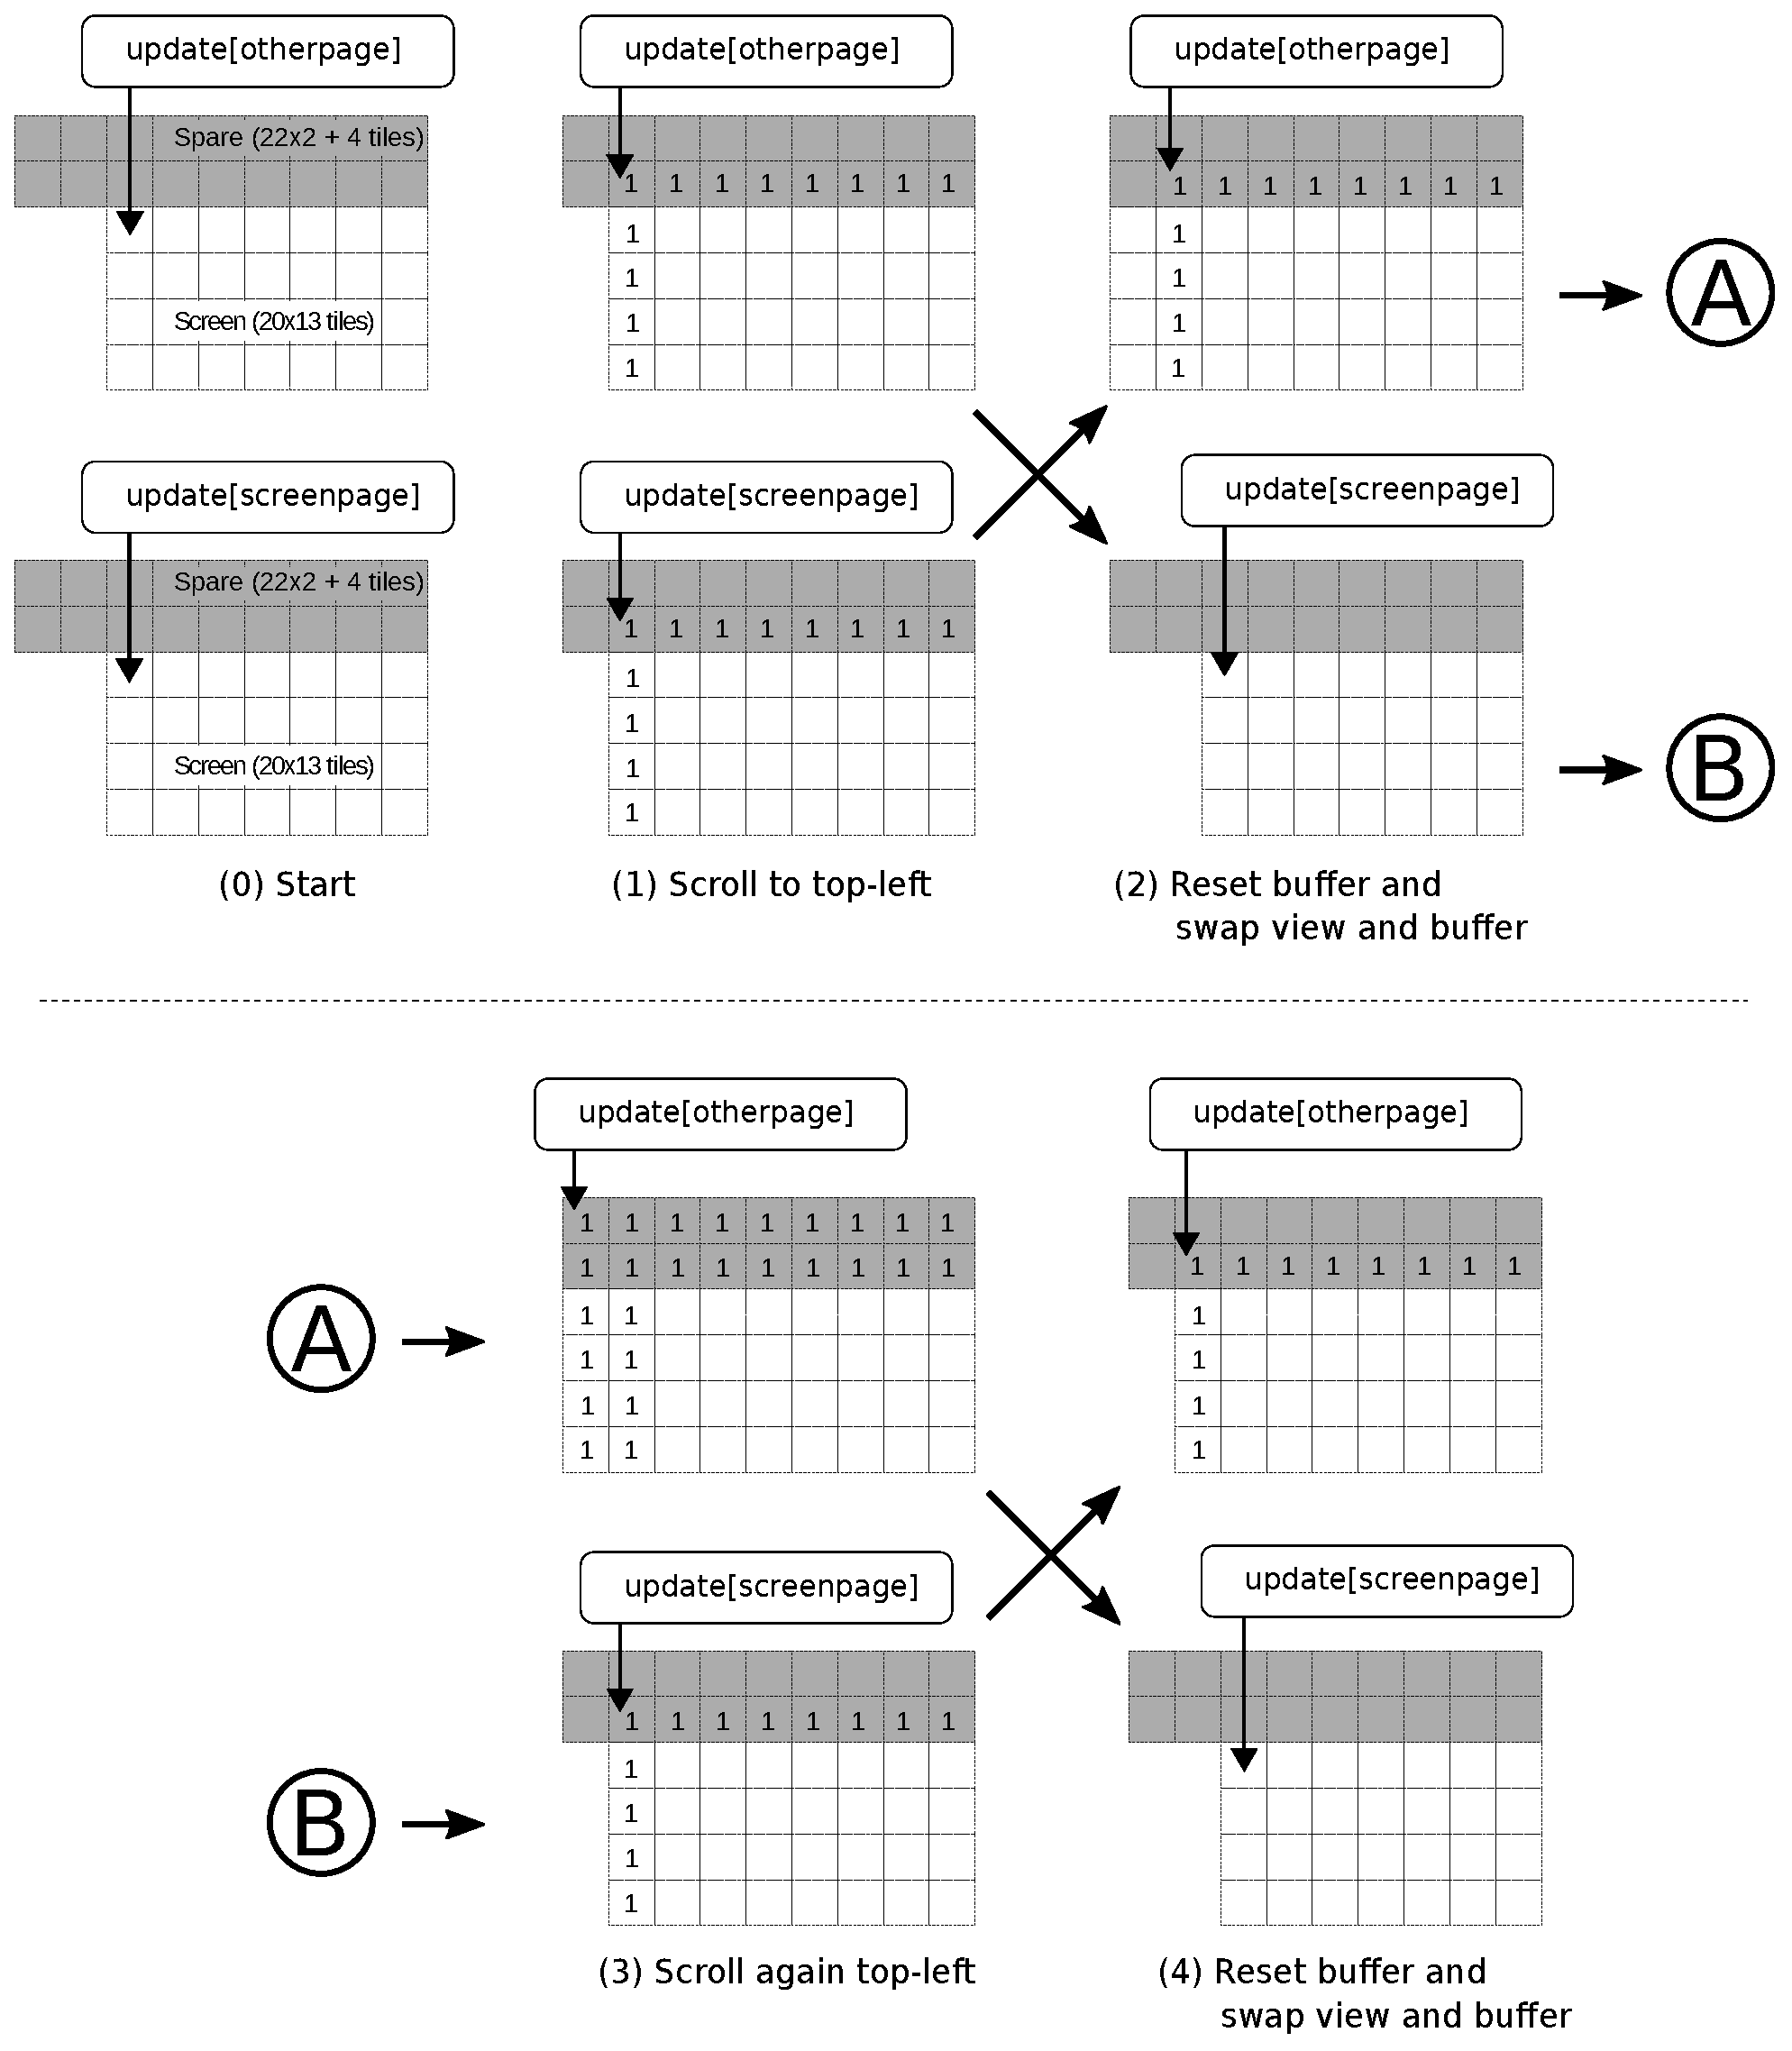
\includegraphics[width=\textwidth]{imgs/drawings/buffer_tile_move.eps}
  \caption{scroll to top-left tile}
  \label{fig:buffer_tile_move_1}
\end{figure}
Now, if the screen is again scrolling to the top-left one can see why there is a need for the 2\textsuperscript{nd} row in the buffer. After this cycle the \cw{*update[otherpage]} pointer is cleared and resetted as shown in the last illustration of Figure \ref{fig:buffer_tile_move_1}.\\
\pagebreak





\section{Actors and sprites}

\subsection{A.I.}
To simulate enemies, some objects are allowed to "think" and take actions like walking,
shooting or emitting sounds. These thinking objects are called "actors".
Actors are programmed via a state machine. They can be aggressive (chase you), just running in any direction, or dump (throwing things at you). To model their behavior, all enemies have an associated state:
\begin{itemize}
  \item Chase Keen
  \item Smash Keen
  \item Shoot projectile
  \item Climb and slide from pole
  \item Walking around
  \item Turn into flower
  \item Special Boss (Boobus)
\end{itemize}
\par

Each state has associated think, reaction and contact method pointers. There is also a next
pointer to indicate which state the actor should transition to when the current state is completed.\\
\par
\begin{minipage}{\textwidth}
  \lstinputlisting[language=C]{code/statetype.c}
\end{minipage}
\label{state_type}
\par

All actors have a state chain, as example the tater trooper.\\
\par
\begin{minipage}{\textwidth}
\lstinputlisting[language=C,style=mystyle,basicstyle=\small]{code/s_grdchase.c}
\end{minipage}
\par
All types of enemies (including Boobus) have their own state machine. They often share
the same reactions (e.g. WalkReact and ProjectileReact), but often have their own thinking state.

\subsection{Drawing Sprites}
\label{section:draw_sprites}
Once the state of the actor is updated, it is time to render the actor on the screen. This is done using sprites and contains the following steps:
\begin{enumerate}
\item Update the state and move actors within the active region.
\item Determinate if a actor has changed or moved
\item Update the actor by removing and drawing sprites to it's new position
\end{enumerate}

Unlike many game consoles such as Nintendo, the concept of sprites did not exists on the EGA card, so again the team needs to write their own solution. As explained in Section \ref{section:asset_file_structure} (Page \pageref{table:spritetable}, table \ref{table:spritetable}) each sprite asset contains additional information which is illustrated in Figure \ref{fig:sprite_structure}.\\
\begin{figure}[H]
  \centering
  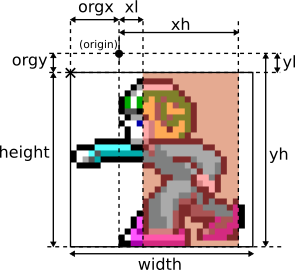
\includegraphics[width=0.6\textwidth]{imgs/drawings/sprite.png}
  \caption{sprite structure}
  \label{fig:sprite_structure}
\end{figure}

All global movement takes place from the origin. The origin \cw{(orgx,orgy)} defines the top-left position of the sprite. Together with the width and height it defines the boundaries of the sprite. The parameters \cw{xl, xh, yl and yh} define the hit box of the sprite, which is used to detect collisions.\\

\begin{table}[H]
  \begin{tabularx}{\textwidth}[c]{lXXXXXXXXX}
  \hline
  \textbf{index} & \textbf{width} & \textbf{height} & \textbf{orgx} & \textbf{orgy}
    & \textbf{xl} & \textbf{yl} & \textbf{xh} & \textbf{yh} & \textbf{shift} \\ \hline
  0  &   3  &   24  &   0  &   0  &   0  &   0  &   368  &   368  &   4 \\
  1  &   3  &   32  &   0  &   0  &   64  &   0  &   304  &   496  &   4 \\
  2  &   3  &   30  &   0  &   16  &   64  &   0  &   304  &   496  &   4 \\
  3  &   3  &   30  &   0  &   32  &   64  &   48  &   304  &   496  &   4 \\
  4  &   3  &   32  &   0  &   0  &   64  &   0  &   304  &   496  &   4 \\
  5  &   3  &   30  &   0  &   32  &   64  &   48  &   304  &   496  &   4 \\
 ...  &   ...  &   ...  &   ...  &   ...  &   ...  &   ...  &   ...  &   ...  &   ... \\
 296  &   12  &   103  &   -128  &   0  &   256  &   128  &   752  &   1648  &   4\\
  \end{tabularx}
  \caption{content of spritetable[] in the \cw{KDREAMS.EGA} asset file.}
  \label{table:spritetable}
\end{table}

As each sprite can float freely over the screen, here also bitshifted sprites are used to position the sprite on a byte-aligned memory layout (as explained in section \ref{section:bitshifting} on page \pageref{section:bitshifting}). The value in the shift column defines the amount of steps the sprite has to be shifted within 8 pixels. A value of 4 means the sprite is shifted in 4 steps with a 2 pixel interval.\\ 

\begin{figure}[H]
  \centering
  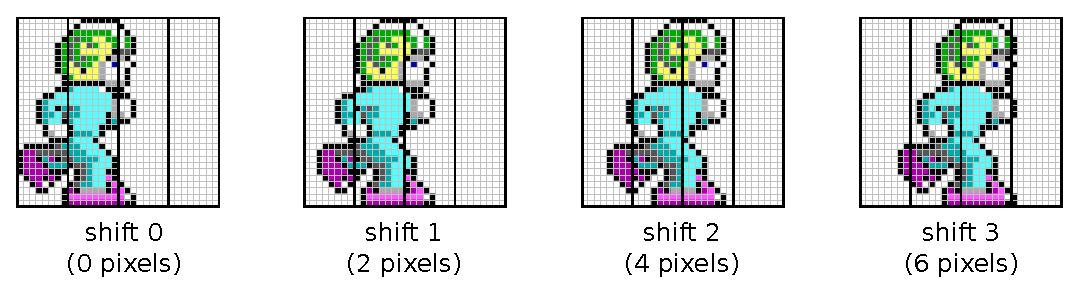
\includegraphics[width=\textwidth]{imgs/drawings/sprite_shift.eps}
  \caption{Sprite shifted in 4 steps.}
  \label{fig:sprite_shift}  
\end{figure}
\par
Displaying the correct shifted sprite is as simple as below.
\\
\par
\begin{minipage}{\textwidth}
  \lstinputlisting[language=C]{code/sprite_shift.c}
\end{minipage}
\label{state_type}
\par


\subsection{Clipping}
\label{section:clipping}
Before drawing a sprite on the screen, the engine determines if the boundaries of a sprite are hitting a wall or floor. This is called clipping and ensures an actor doesn't fall through a floor or walks through a vertical wall. To define whether a tile is a wall or floor, a tile is enriched with tile information, as explained in section \ref{section:foreground_tile_info} on page \pageref{section:foreground_tile_info}. Each foreground tile contains a \cw{NORTHWALL}, \cw{SOUTHWALL}, \cw{EASTWALL} and \cw{WESTWALL}, as explained in section \ref{section:foreground_tile_info}. A number greater than 0 means the tile is a wall or floor when approaching from a given direction. 

\begin{figure}[H]
\centering
\begin{subfigure}{.5\textwidth}
  \centering
  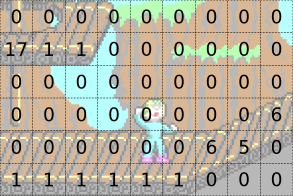
\includegraphics[width=.9\textwidth]{screenshots_300dpi/game/clip_tinf_1.png}
  \caption{Wall type map NORTHWALL}
  \label{fig:clip_tinf_n}
\end{subfigure}%
\begin{subfigure}{.5\textwidth}
  \centering
  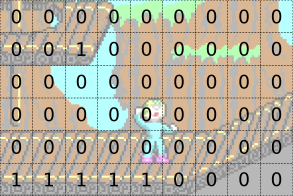
\includegraphics[width=.9\textwidth]{screenshots_300dpi/game/clip_tinf_east.png}
  \caption{Wall type map EASTWALL}
  \label{fig:clip_tinf_e}
\end{subfigure}
\caption{Foreground tile clipping information.}
\label{fig:clip_tinf}
\end{figure}

\par
When a sprite, moving from right to left, is hitting a wall on the left side, it will update the sprite movement to ensure the sprite clips to the eastwall of the left tile as illustrated in Figure \ref{fig:clipping_east}. The east/west wall clipping logic is covered by \cw{ClipToEastWalls()} and \cw{ClipToWestWalls()} functions. \\

\begin{figure}[H]
  \centering
  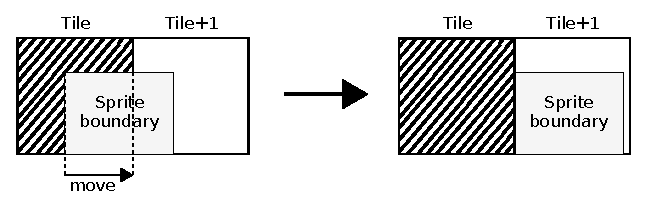
\includegraphics[width=\textwidth]{imgs/drawings/clipping_east.eps}
  \caption{Clipping to east wall when moving from the west.}
  \label{fig:clipping_east}  
\end{figure}

\par
\begin{minipage}{\textwidth}
  \lstinputlisting[language=C]{code/clip_east_wall.c}
\end{minipage}
\label{wallclip_array}
\par
For clipping top and bottom the engine also needs to take walking on slopes into account. After the sprite is clipped to the top or bottom of the wall tile, an offset can be applied to move a sprite up or down a slope. The offset is defined by a lookup table, where the midpoint pixel of the sprite (0-15) and the wall type from the map defines the offset.

\begin{figure}[H]
  \centering
  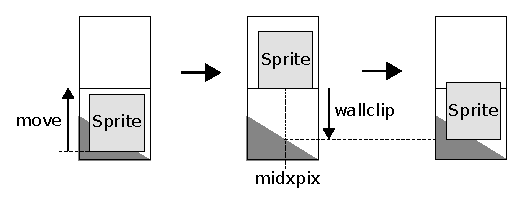
\includegraphics[width=\textwidth]{imgs/drawings/clipping_north.eps}
  \label{fig:clipping_north}
  \caption{Clipping north wall with slope.}
\end{figure}



\begin{minipage}{\textwidth}
  \lstinputlisting[language=C,style=mystyle,basicstyle=\scriptsize]{code/wallclip_array.c}
\end{minipage}
\label{wallclip_array}
\par
\begin{figure}[H]
  \centering
  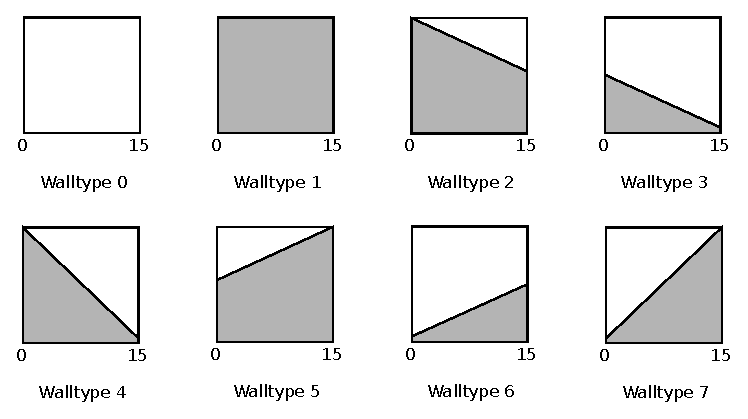
\includegraphics[width=\textwidth]{imgs/drawings/walltype.eps}
  \label{fig:walltype}
  \caption{Eight different walltypes (slopes) defined.}
\end{figure}



\par
\begin{minipage}{\textwidth}
  \lstinputlisting[language=C]{code/clip_north_wall.c}
\end{minipage}
\label{wallclip_array}
\par

\subsection{Priority of tiles and sprites on screen}
The normal screen build is as follows:
\begin{enumerate}
  \item Draw the background tile.
  \item Draw the masked foreground tile.
  \item Draw the sprites on top of both the background and foreground tiles.
\end{enumerate}

If multiple sprites are displayed on the same tile, each sprite is given a priority 0-3 to define the order of drawing. A sprite with a higher priority number is always displayed on top of lower priority sprites. As sprites are always displayed on top of tiles, this is causing unnatural situation when Commander Keen is climbing through a  hole as illustrated in Figure \ref{fig:draw_layers}.\\

\begin{figure}[H]
\begin{subfigure}{.25\textwidth}
  \centering
  
\includegraphics[width=.9\textwidth]{screenshots_300dpi/game/tile_composite_1.png}
  \caption{Background tile.}
\end{subfigure}%
\begin{subfigure}{.25\textwidth}
  \centering
  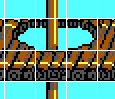
\includegraphics[width=.9\textwidth]{screenshots_300dpi/game/tile_composite_2.png}
  \caption{Foreground tile.}
\end{subfigure}
\begin{subfigure}{.25\textwidth}
  \centering
  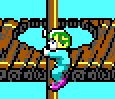
\includegraphics[width=.9\textwidth]{screenshots_300dpi/game/tile_composite_3.png}
  \caption{Sprite on top.}
\end{subfigure}
\caption{Unnatural situation where Commander Keen is in front of a hole.}
\label{fig:draw_layers}
\end{figure}
\par

To draw sprites 'inside' a foreground tile, a small trick is used by introducing a priority foreground tile. As explained in section \ref{section:foreground_tile_info} each foreground tile is enriched with INTILE ('inside tile') information. If the highest bit (\cw{80h}) of INTILE is set, this foreground tile has a higher priority than sprites with a priority 0, 1 or 2. So when drawing the tiles and sprites the following drawing order is applied:
\begin{enumerate}
  \item Draw the background tile.
  \item Draw the masked foreground tile.
  \item Draw sprites with priority 0, 1 and 2 (in that order) and mark the corresponding tile in the tile buffer array with '3' as illustrated in Figure \ref{fig:kc1_3_tile_update_sprite} on page \pageref{fig:kc1_3_tile_update_sprite}.
  \item Scan the tile buffer array for tiles marked with '3'. If the corresponsing foreground INTILE high bit is set, redraw the masked foreground tile.
  \item Finally, draw sprites with priority 3. These sprites are always on top of everything.
\end{enumerate}
\par
The priority foreground tiles are updated in the \cw{RFL\_MaskForegroundTiles()} function.\\

\begin{figure}[H]
\centering
\begin{subfigure}[t]{.245\textwidth}
  \centering
  
\includegraphics[width=.9\textwidth]{screenshots_300dpi/game/tile_composite_1.png}
  \caption{Background tile.}
\end{subfigure}%
\begin{subfigure}[t]{.245\textwidth}
  \centering
  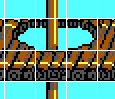
\includegraphics[width=.9\textwidth]{screenshots_300dpi/game/tile_composite_2.png}
  \caption{Foreground tile.}
\end{subfigure}
\begin{subfigure}[t]{.245\textwidth}
  \centering
  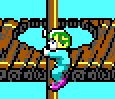
\includegraphics[width=.9\textwidth]{screenshots_300dpi/game/tile_composite_3.png}
  \caption{Sprite on top.}
\end{subfigure}
\begin{subfigure}[t]{.245\textwidth}
  \centering
  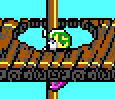
\includegraphics[width=.9\textwidth]{screenshots_300dpi/game/tile_composite_4.png}
  \caption{Redraw masked foreground tile.}
\end{subfigure}
\caption{Draw sprite inside a tile, by redrawing foreground tile.}
\label{fig:clip_tinf}
\end{figure}

\par
\begin{minipage}{\textwidth}
  \lstinputlisting[language={[x86masm]Assembler}]{code/mask_foreground_tile.asm}
\end{minipage}
\label{mask_foreground_tile}
\par


\end{document}